
\label{sec:trigo}
\section{Trigonometry review}
\begin{theorem}
    {Trigonometric identities}
    \begin{enumerate}
        \item $\sin^2x+\cos^2x=1$
        \item $\tan x=\frac{\sin x}{\cos x}$
        \item $\csc x=\frac{1}{\sin x}$
        \item $\sec x=\frac{1}{\cos x}$
        \item $\cot x=\frac{1}{\tan x}$
        \item $\sin 2x=2\sin x\cos x$
        \item $\cos 2x=\cos^2x-\sin^2x$
        \item $\tan 2x=\frac{2\tan x}{1-\tan^2x}$
        \item $\sin(x\pm y)=\sin x\cos y\pm\cos x\sin y$
        \item $\cos(x\pm y)=\cos x\cos y\mp\sin x\sin y$
        \item $\tan(x\pm y)=\frac{\tan x\pm\tan y}{1\mp\tan x\tan y}$
        \item $1 + tan^2x = sec^2x$
        \item $1 + cot^2x = csc^2x$
    \end{enumerate}
\end{theorem}
Related: \hyperref[sec:integrationtech]{Techniques of integration}

\section{Derivatives}
\begin{definition}
    {First principle}
    The first principle is the definition of the derivative of a function $f(x)$ at $x=a$:
    \[f'(x) = \frac{d}{dx} f(x)=\lim_{h\to 0}\frac{f(x+h)-f(x)}{h}\]
    Note the notation of \textit{prime} ($'$), which denotes the derivative against $x$ for any function primed.
\end{definition}

\begin{theorem}
    {Differentiability}
    The function is differentiable at $x=a$ if:
    \[\lim_{x\to a^-}f'=\lim_{x\to a^+}f'\]
    Use first principle if the function is cased.
\end{theorem}

\subsection{Differentiation formulas and rules}
\begin{knBox}
    {Basic formulas}
    \begin{itemize}
        \item We can differentiate individual items: $\displaystyle {\left( {f \pm g} \right)^\prime } = f' \pm g'$
        \item We can factor out a multiplicative constant: $\displaystyle {\left( {cf} \right)^\prime } = cf'$
        \item Derivative of a constant is 0: $\frac{d}{dx}k = 0$
        \item Power rule: $\frac{d}{dx}x^n = nx^{n-1}$
    \end{itemize}
\end{knBox}
\begin{minipage}{0.65\textwidth}
    \begin{theorem}
        {Chain rule}
        Shorthand: \textbf{d}1x2 + \textbf{d}2x1
        \[(u(v))'=u'(v)v'\quad\quad\text{or}\quad\quad\frac{dy}{dx}=\frac{dy}{du}\frac{du}{dx}\]
    \end{theorem}
    \begin{theorem}
        {Product rule}
        Shorthand: \textbf{d} from outside to inside
        \[(uv)' = uv' + vu'\quad\quad\text{or}\quad\quad\frac{d}{dx}(uv)=u\frac{dv}{dx}+v\frac{du}{dx}\]
    \end{theorem}
    \begin{theorem}
        {Quotient rule}
        Shorthand: move lower \textbf{d} upper - \textbf{d} lower x upper, lower square
        \[(\frac{u}{v})'=\frac{vu'-uv'}{v^2}\quad\quad\text{or}\quad\quad\frac{d}{dx}(\frac{u}{v})=\frac{v\frac{du}{dx}-u\frac{dv}{dx}}{v^2}\]
    \end{theorem}
\end{minipage}
\hfill
\begin{minipage}{0.28\textwidth}
    \begin{table}[H]
        \begin{tabular}{rcc}
                & $f(x)$        & $f'(x)$                \\ \hline
            1.  & $a^x$         & $\ln{a}\cdot a^x$      \\ \arrayrulecolor{lightgray}\hline
            2.  & $e^{kx}$      & $ke^{kx}$              \\ \arrayrulecolor{lightgray}\hline
            3.  & $\ln{kx}$     & $x^{-1}$               \\ \arrayrulecolor{lightgray}\hline
            4.  & $|x|$         & $\frac{|x|}{x}$        \\ \arrayrulecolor{lightgray}\hline
            5.  & $\sin kx$     & $k\cos kx$             \\ \arrayrulecolor{lightgray}\hline
            6.  & $\cos kx$     & $-k\sin kx$            \\ \arrayrulecolor{lightgray}\hline
            7.  & $\tan kx$     & $k\sec^2 kx$           \\ \arrayrulecolor{lightgray}\hline
            8.  & $\csc x$      & $-\csc x \cot x$       \\ \arrayrulecolor{lightgray}\hline
            9.  & $\sec x$      & $\sec x \tan x$        \\ \arrayrulecolor{lightgray}\hline
            10. & $\cot x$      & $-\csc^2x$             \\ \arrayrulecolor{lightgray}\hline
            11. & $\sin^{-1} x$ & $(\sqrt{1-x^2})^{-1}$  \\ \arrayrulecolor{lightgray}\hline
            12. & $\cos^{-1} x$ & $-(\sqrt{1-x^2})^{-1}$ \\ \arrayrulecolor{lightgray}\hline
            13. & $\tan^{-1} x$ & $(1+x^2)^{-1}$
        \end{tabular}
    \end{table}
\end{minipage}

% Note that the trigo derivatives can be extended to hyperbolic trigo functions, with the except of $\frac{d}{dx}\text{sech} u=-\text{sech} u\tanh u$.

\subsection{Techniques of differentiation}
\begin{knBox}
    {Parametric differentiation}
    For a parametric equation $y=f(t)$ and $x=g(t)$:
    \[\frac{dy}{dx}=\frac{dy}{dt}\div \frac{dx}{dt}\]
\end{knBox}
\begin{knBox}
    {Inverse functions}
    $f^{-1}(x): f(x)\leftrightarrow x$ (switch $x$ and $y$).
    \begin{enumerate}
        \item Inverse functions only exists in the domain of $f$ where $f$ is \emph{bijective} (one-to-one and onto). This means that the domain where $f$ gives unique values is the range of $f^{-1}$.
        \item The range of $f$ is the domain of $f^{-1}$.
        \item The domain of $f$ is the range of $f^{-1}$.
    \end{enumerate}
\end{knBox}
\begin{theorem}
    {Derivative of Inverse functions}
    At $c$, we first find $f'(x)$ and the value of $f^{-1}(c)$, then we apply the formula to find the value of $f^{-1'}(c)$:
    \[f^{-1'}(c)=\frac{1}{f'(f^{-1}(c))}\]
    $f^{-1}(c)$ can be found by solving $f(x)=c$.
\end{theorem}

\begin{knBox}
    {Implicit differentiation}
    Differentiate all $xy$, add $y'$ behind all differentiations of $y$.
    \tcblower
    To find $y'$ for $y^2=x^2+\sin(xy)$:
    \begin{align*}
        y^2                                     & =x^2+\sin(xy)                      \\
        2yy'                                    & =\frac{d}{dx}(\sin(xy))            \\
        2yy'                                    & =2x+\cos(xy)(xy'+y)                \\
        \text{Then we simply collect terms of } & y'                                 \\
        y'                                      & =\frac{2x+y\cos(xy)}{2y-x\cos(xy)}
    \end{align*}
    To find the second derivative $y''$, differentate the expression and substitute $y'$ back in.
\end{knBox}
\begin{knBox}
    {Logarithmic differentiation}
    To differentiate a function to the power of another function, we can take the logarithm of the function, then differentiate.
    \begin{align*}
        (f^g)'&=(e^{g\ln f}) \\
        & = (g\ln f)'e^{g\ln f}
    \end{align*}
    \tcblower
    To find $\frac{dy}{dx}$ for $y=x^x$:
    \begin{align*}
        y & =  e^{x\ln x} \\
         & = e^{x\ln x}(\ln x+x\frac{1}{x}) \\
            & = x^x(\ln x+1)
    \end{align*}
\end{knBox}
\label{sec:lhr}
\begin{theorem}
    {L'Hopital's rule}
    For any $a\in [\mathds{R}, \pm\infty]$, if $\lim_{x\to a}(\frac{f}{g})$ is in \hyperref[sec:indeterminate]{indeterminate form} after substitution, we can conclude:
    \[\lim_{x\to a}(\frac{f}{g})=\lim_{x\to a}(\frac{f'}{g'})\]
    \tcblower
    To find $\lim_{x\to-\infty}xe^x$, we first check if the limit is indeterminate, then we can apply the rule:
    \begin{align*}
        \lim_{x\to-\infty}xe^x & \implies \infty\times0                                      \\
        \lim_{x\to-\infty}xe^x & = \lim_{x\to-\infty}\frac{x}{e^{-x}}                        \\
                               & = \lim_{x\to-\infty}\frac{1}{-e^{-x}}\text{ (rule applied)} \\
                               & = 0
    \end{align*}
\end{theorem}

\subsection{Important theorems}
\begin{theorem}
    {Mean value theorem (MVT)}
    For $f(x)$ that is \emph{continuous} in $[a,b]$ and \emph{differentiable} in $(a,b)$:
    \[f'(c)=\frac{f(b)-f(a)}{b-a},\quad c\in(a,b)\]
    \tcblower
    The theorem tells us that, in described conditions, there must be a point $c$ where the slope of the \emph{tangent line} is equal to the slope of the line from $a\to b$ (secant line).
    \begin{figure}[H]
        \centering
        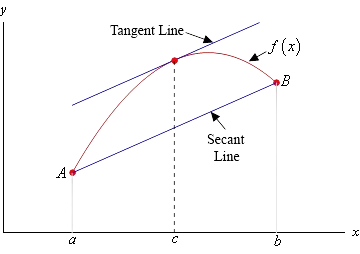
\includegraphics[width=0.4\textwidth]{./img/mvt.png}
        \caption*{\tiny\textit{\color{gray}Source: https://tutorial.math.lamar.edu/Classes/CalcI/MeanValueTheorem.aspx}}
    \end{figure}
\end{theorem}
\begin{theorem}
    {Rolle's theorem}
    For $f(x)$ that is \emph{continuous} in $[a,b]$ and \emph{differentiable} in $(a,b)$:
    \[\forall\ f(a)=f(b)\text{  there exists  }f'(c)=0,\quad c\in(a,b)\]
    \begin{center}
        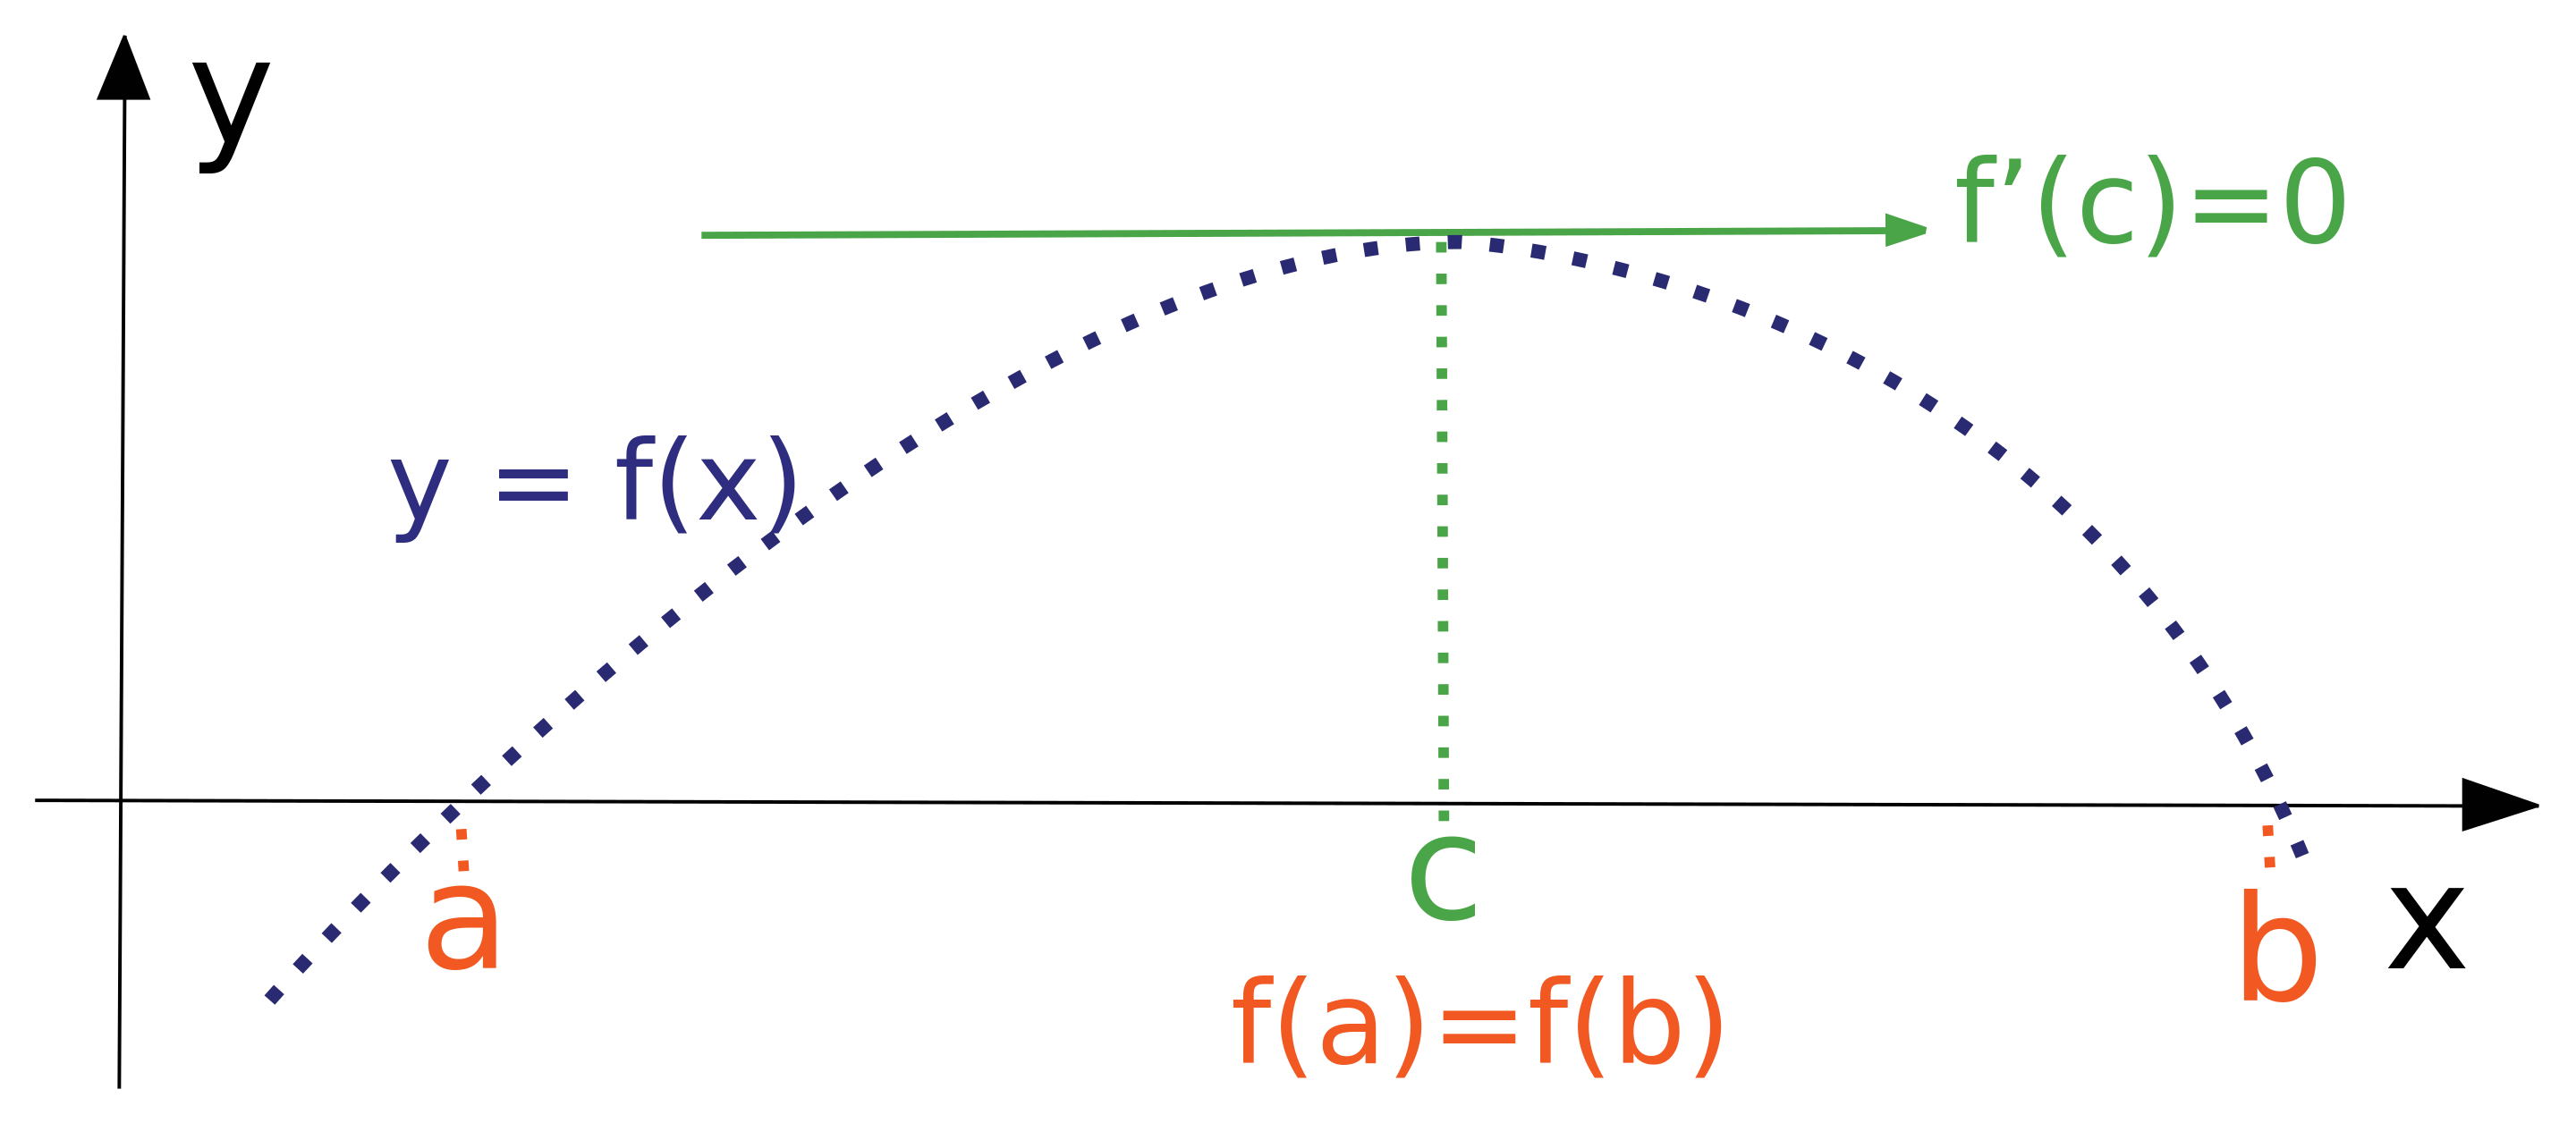
\includegraphics[width=0.3\textwidth]{./img/rt.png}
    \end{center}
    \tcblower
    For $F'=f$, if $F$ has 4 roots, then $f$ has 3 roots.
\end{theorem}


\subsection{Extremum points}
\begin{definition}
    {Critical and inflection points}
    A \textbf{critical point} is a point where $f'(x)=0$ or undefined, or the end-points of the domain if inclusive.

    An \textbf{inflection point} is a point where $f''(x)=0$ or undefined, that the \hyperref[sec:concavity]{concavity} of the function changes.
\end{definition}
\begin{definition}
    {Max/minimum points}
    The \textbf{absolute maximum/minimum points} are the points where the function has the largest/smallest value in the entire domain.

    The \textbf{local maximum/minimum points} are the points where the function has the largest/smallest value in a small interval around the point.
\end{definition}
% \begin{theorem}
%     {Extreme value theorem}
%     For $f(x)$ that is \emph{continuous} in $[a,b]$, there must be both an abs maximum and minimum point.
%     \tcblower
%     To find the absolute extremas of $f(x)$ in $[a,b]$, we can:
%     \begin{enumerate}
%         \item Verify that $f(x)$ is continuous in $[a,b]$
%         \item Find all critical points in $[a,b]$
%         \item Evaluate the critical points as well as the end points of the interval
%     \end{enumerate}
% \end{theorem}

\subsection{Determining shape of graph}

\label{sec:concavity}
\begin{definition}
    {Concavity}
    Concavity is the direction of the curve, and can be described by the values of $f'$ and $f''$:
    \begin{table}[H]
        \begin{tabular}{lcccc}
            $f''$ & $-$                                                                & $+$                                                                & $+$                                                               & $-$                                                              \\
            $f'$  & $-$                                                                & $+$                                                                & $-$                                                               & $+$                                                              \\
            $f$   & 
\includegraphics[width=0.3cm,origin=c, angle=270]{./img/arrow.png} & 
\includegraphics[width=0.3cm,origin=c, angle=180]{./img/arrow.png} & 
\includegraphics[width=0.3cm,origin=c, angle=90]{./img/arrow.png} & 
\includegraphics[width=0.3cm,origin=c, angle=0]{./img/arrow.png}
        \end{tabular}
    \end{table}
    Note: Arrows goes clock-wise.
\end{definition}

\begin{table}[H]
    \begin{tabular}{rll}
            & Step                                 & Expression                                                                                                                                                                                                                                                                              \\ \hline
        1.  & Determine domain of function         &                                                                                                                                                                                                                                                                                         \\
        2.  & Special points without continuity?   &                                                                                                                                                                                                                                                                                         \\
        3.  & Axis intercepts                      & $(f(x)=0, 0)\ (0, f(0))$                                                                                                                                                                                                                                                                \\
        4.  & Critical points                      & $f'(x)=0$ or undefined                                                                                                                                                                                                                                                                  \\
        5.  & Point maxima?                        & $+f''(x)$ or $-f''(x)$                                                                                                                                                                                                                                                                  \\
        6.  & Inflection points                    & $f''(x)=0$ or undefined                                                                                                                                                                                                                                                                 \\
        7.  & Horizontal asymptotes                & $\lim_{x\to\pm\infty}f(x)=n?$                                                                                                                                                                                                                                                           \\
        8.  & Vertical asymptotes                  & $\lim_{x\to a^\pm}f(x)=\pm\infty?$                                                                                                                                                                                                                                                      \\
        9.  & Area strictly increasing/decreasing? & $f'(x)>0$ or $f'(x)<0$                                                                                                                                                                                                                                                                  \\
        10. & Area concavity?                      & $-++-/-+-+/$
\includegraphics[width=0.3cm,origin=c, angle=270]{./img/arrow.png}  
\includegraphics[width=0.3cm,origin=c, angle=180]{./img/arrow.png}  
\includegraphics[width=0.3cm,origin=c, angle=90]{./img/arrow.png}  
\includegraphics[width=0.3cm,origin=c, angle=0]{./img/arrow.png} \\
    \end{tabular}
\end{table}

Related: \hyperref[sec:asymptotes]{Definition of asymptotes}

\begin{knBox}
    {Higher derivatives}
    Derivatives of higher order (e.g. $f''(x), f'''(x)$) can be expressed as $f^{(n)}(x)$
\end{knBox}

\section{Integrals}
\subsection{Definite integrals}
\begin{definition}
    {Signed areas}
    Signed area is the area between the curve and the x-axis, where the area above the x-axis is positive and below is negative.
\end{definition}
\begin{knBox}
    {Properties of definite intergrals}
    \begin{enumerate}
        \item $\int_{a}^{b}f(x)dx=-\int_{b}^{a}f(x)dx$
        \item $\int_{a}^{a}f(x)dx=0$
        \item $\int_{a}^{b}f(x)dx+\int_{b}^{c}f(x)dx=\int_{a}^{c}f(x)dx$
        \item $\int_{a}^{b}kf(x)dx=k\int_{a}^{b}f(x)dx$
        \item $\int_{a}^{b}(f(x)\pm g(x))dx=\int_{a}^{b}f(x)dx\pm\int_{a}^{b}g(x)dx$
    \end{enumerate}
\end{knBox}
\subsection{Fundamental theorem of calculus}
\begin{theorem}
    {Fundamental theorem of calculus (FTC)}
    If $f(x)$ is continuous in $[a,b]$, then:
    \[\int_{a}^{b}f(x)dx=F(b)-F(a)\]
    Where $F(x)$ is the definite integral of $f(x)$.
\end{theorem}
\begin{theorem}
    {Second fundamental theorem of calculus}
    If $f(x)$ is continuous in $[a,b]$, then:
    \[\frac{d}{dx}\int_{a}^{x}f(t)dt=f(x)\]
    \tcblower
    Find $g'(x)$ for $g(x)=\int_1^{x^2}\cos t\ dt$:

    We first define $G(u)=\int_1^{u}\cos t\ dt$, then we can apply the chain rule:
    \begin{align*}
        g'(x) & =(G(x^2))' \\&=G'(x^2)\cdot2x\\&=\cos x^2\cdot2x
    \end{align*}
\end{theorem}
\begin{knBox}
    {Cases of area 0}
    For $\int^{b}_{a}f(x)dx$:
    \begin{itemize}
        \item If $b=a$, then the area is 0 (no width)
        \item If $f(x)=f(-x)$ and $a=-b$, then the area is 0 (symmetry)
    \end{itemize}
\end{knBox}
\begin{theorem}
    {Limit of Riemann sums}
    We can convert a limit to infinity of a Riemann sum to a definite integral:
    \[\lim_{n\to\infty}\sum_{i=1}^{n}f(a+i\Delta x)\Delta x=\int_{0}^{b}f(a+x)dx,\quad\Delta x=\frac{b-a}{n}\]
    Some properties of summation:
    \begin{enumerate}
        \item $x\sum f(x) = \sum x f(x)$
        \item $\sum_{i=1+n} f(x, i), \text{let }k=i-n\to\sum_{k=1}^{n}f(x, k+n)$
    \end{enumerate}
\end{theorem}

\label{sec:integrationtech}
\subsection{Techniques of integration}
\begin{knBox}
    {Overview}
    \begin{itemize}
        \item By \hyperref[sec:intsub]{\textbf{substitution}}: “sub $g(x)\to u$, find $du$ and replace all functions of $x(dx)$ with $u(du)$”
        \item By \hyperref[sec:intpart]{\textbf{part}}: “$\int ab=a\int b-\int (a'\times \int b)$”
        \item By \textbf{joining recurring parts}: “$\int ab=f(ab)+\int ab\to 2\int ab = f(ab)$”
        \item By \textbf{partial fractions}: “$\frac{k}{f(x)g(x)}=\frac{A}{f(x)}+\frac{B}{g(x)}$”
        \item By \hyperref[sec:inttrigo]{\textbf{trigonometric identities}}
        \item By \textbf{multiplying fractions by one}: “Multiplying $\frac{\sec^2x}{\sec^2x}$ to fit trigo form”
    \end{itemize}
\end{knBox}

\label{sec:intsub}
\begin{theorem}
    {Integration by substitution}
    For $\int f(g)g'\:dx$:
    \begin{enumerate}
        \item Let $u=g$
        \item Find $du=g'dx$
        \item Change limits in terms of $u$ if definite
        \item Replace all $g\to u$ and $g'dx\to du$
        \item Integrate, then subsitute $u\to g$
    \end{enumerate}
\end{theorem}

\label{sec:intpart}
\begin{theorem}
    {Integration by parts}
    \[\int ab=a\int b-\int (a'\times \int b)\]
    \emph{Tips:}
    Let $a$ (differentiating term) to the first term you see on the list:
    \begin{enumerate}
        \item \textbf{L}ogarithmic
        \item \textbf{I}nverse trigo
        \item \textbf{A}lebratic (polynomial)
        \item \textbf{T}rigo
        \item \textbf{E}xponential
    \end{enumerate}
\end{theorem}
\begin{knBox}
    {Deriving the IBP formula}
    The formula is derived from the product rule of differentiation:
    \begin{align*}
        (ab)'    & = a'b + b'a                     \\
        b'a      & = (ab)' - a'b                   \\
        \int b'a & = ab - \int a'b                 \\
        \int ab  & =a\int b-\int (a'\times \int b)
    \end{align*}
\end{knBox}

\label{sec:inttrigo}
\begin{knBox}
    {Trigo-identities substitution tips}
    Use the following trigonometric identities to simplify the integral:
    \begin{itemize}
        \item $\sin^2x+\cos^2x=1$
        \item $\sin^2x=\frac{1-\cos2x}{2}$
        \item $\cos^2x=\frac{1+\cos2x}{2}$
        \item $2\sin x\cos x=\sin2x$
        \item $\cos2x=\cos^2x-\sin^2x$
        \item $\sec^2x=1+\tan^2x$
        \item $\csc^2x=1+\cot^2x$
    \end{itemize}
    Use the following substitutions for similar expressions:
    \[
        \text{Expressions of the form }
        \begin{cases}
            a^2-f(x)^2 & \to f(x)=a\sin\theta \\
            a^2+f(x)^2 & \to f(x)=a\tan\theta \\
            f(x)^2-a^2 & \to f(x)=a\sec\theta \\
        \end{cases}
    \]
    Remember that this uses \emph{integration by substitution}, so we need to find $dx$ in terms of $\theta$.
\end{knBox}
\subsection{Solids of revolution}
\begin{definition}
    {Solids of revolution}
    A 3D shape formed by rotating a \emph{region} around an axis.
    \tcblower
    A region is defined by 2 curves and an interval:
    \begin{enumerate}
        \item The vertical region bounded by an outer cruve $R(x)$ and an inner curve $r(x)$.
        \item The inner curve is $y=0$ for the region bounded by the $x$-axis.
        \item The horizontal region is bounded by an interval $x:\ [a, b]$
    \end{enumerate}

    Note that for the methods below, the terms $x$ and $y$ can be \emph{switched} to fit the problem.

    $\{f(x)\to\ \circlearrowright x\}$ denotes using a function of $x$ to find the volume of a solid of revolution around the $x$-axis.
    \begin{enumerate}
        \item If the volume is generated by the rotation about an axis other than the main axes, we can simply \emph{shift} the function to fit the main axes.
        \item If the curves in the given range does not form a closed region with only acute angles, we can \emph{split} the region into multiple parts.
    \end{enumerate}
\end{definition}
\begin{theorem}
    {Volume by Washers (Disk)}
    \[\{f(x)\to\ \circlearrowright x\}:\quad V=\pi\int_{a}^{b}R^2(x)-r^2(x)dx\]
    For rotating about $y=n$: $\forall R/r(x)\to n-R/r(x)$
\end{theorem}
\begin{theorem}
    {Volume by Cylindrical shells}
    \[\{f(x)\to\ \circlearrowright y\}:\quad V=2\pi\int_{a}^{b}[x][R(x)-r(x)]dx\]
    For rotating about $x=n$: $[x]\to [x-n]$
\end{theorem}

\subsection{Arcs and surfaces}
\begin{theorem}
    {Arc length}
    The \emph{arc length} of a curve $y=f(x)$ from $x=a$ to $x=b$ is given by:
    \[L=\int_{a}^{b}\sqrt{1+f'^2(x)}dx\]
    And for parametized equations $x=f(t)$, $y=g(t)$:
    \[L=\int_{a}^{b}\sqrt{f'^2(t)+g'^2(t)}dt\]
    For polar equations $r=f(\theta)$:
    \[L=\int_{a}^{b}\sqrt{r^2+r'^2(\theta)}d\theta\]
\end{theorem}
\begin{theorem}
    {Area surfaces of revolution}
    Used to find the \emph{surface area} generated by rotating a curve along an axis.
    \[\{f(x)\to\ \circlearrowright x\}:\quad A=2\pi\int_{a}^{b}f(x)\sqrt{1+f'^2(x)}dx\]
    And for parametized equations $x=f(t)$, $y=g(t)$:
    \[A=2\pi\int_{a}^{b}g(t)\sqrt{f'^2(t)+g'^2(t)}dt\]
\end{theorem}